\section{Transition Functions of the Alignment Vector $\pmb{x}$}

\label{Appendix_AlignmentFunctions}

The following shows that the vector $x$ returns to its initial state after executing one of the basic moves four times. Here $(\sigma, x)$ is any cube configuration. In this section, only the alignment vector $x$ is considered. The corresponding justification for $\sigma$ can be found in section \ref{Section_EqualityOfmoves}.
\begin{align*}
\forall \ Z \in \{U, D, R, L, F, B\} \ . \ (\sigma, x) \cdot Z^4 = (\sigma, x)
\end{align*}


The vector is changed by the function $\gamma$. This function was defined for each of the basic moves in section \ref{Section_AlignmentOfcubies}.

First, the change in the vector $x$ is examined using the move $R$ as an example. The following figures show the transition functions of the vector entries in the cube:
\begin{figure}[H]
\centering
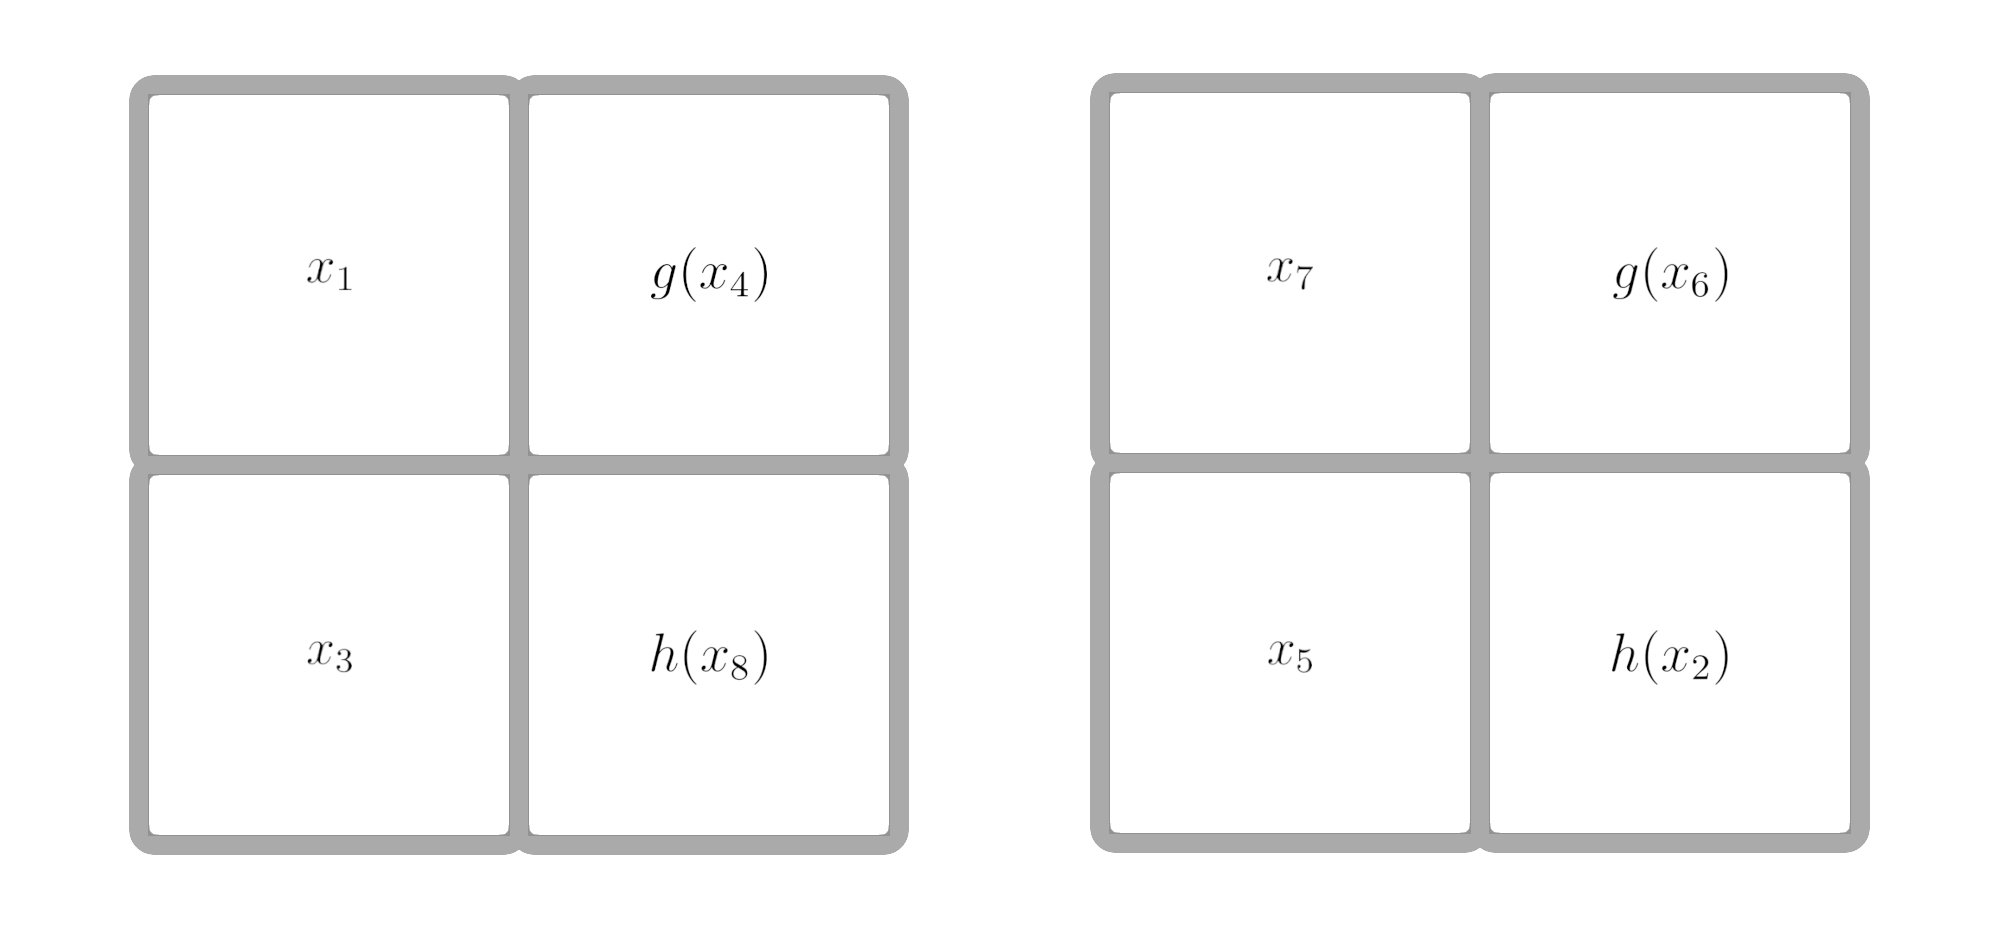
\includegraphics[scale=0.155]{Rhoch1.jpg}
\caption{Vector $x$ to $\gamma_R(x)$}
\end{figure}

\begin{figure}[H]
\centering
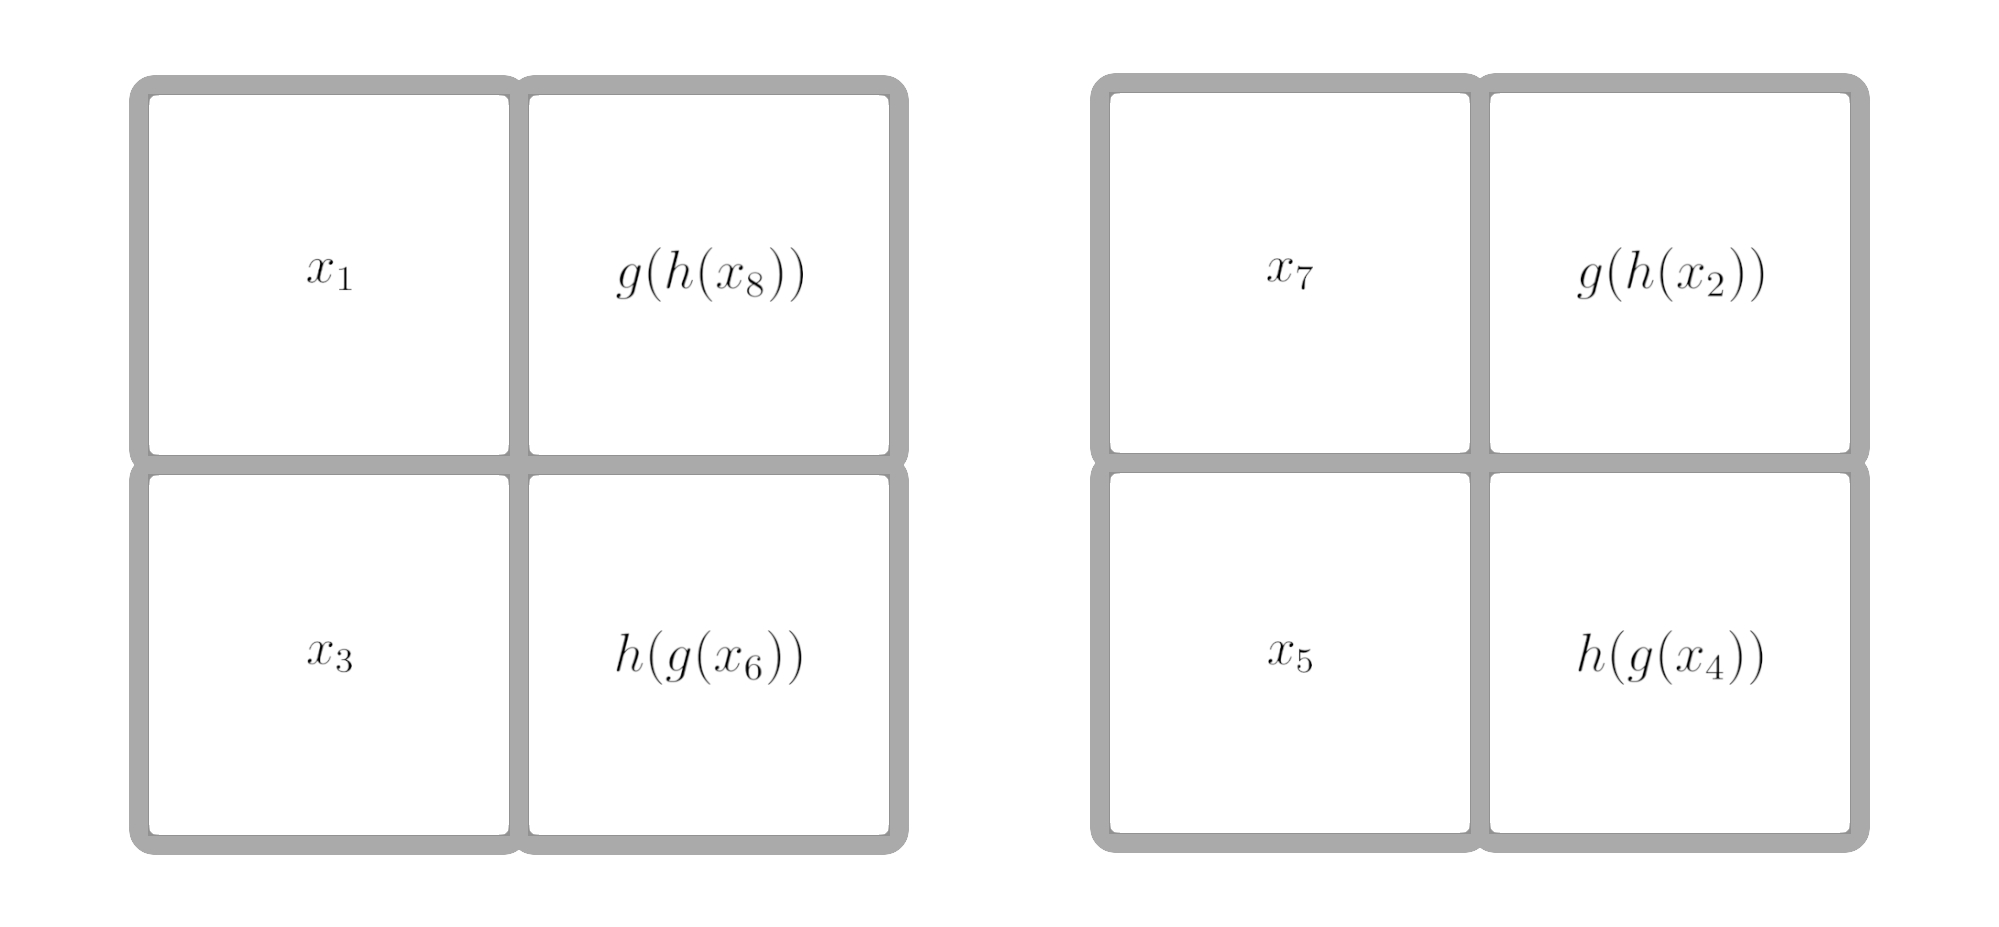
\includegraphics[scale=0.155]{Rhoch2.jpg}
\caption{Vector $x$ to $\gamma_R (\gamma_R(x))$}
\end{figure}
\begin{figure}[H]
\centering
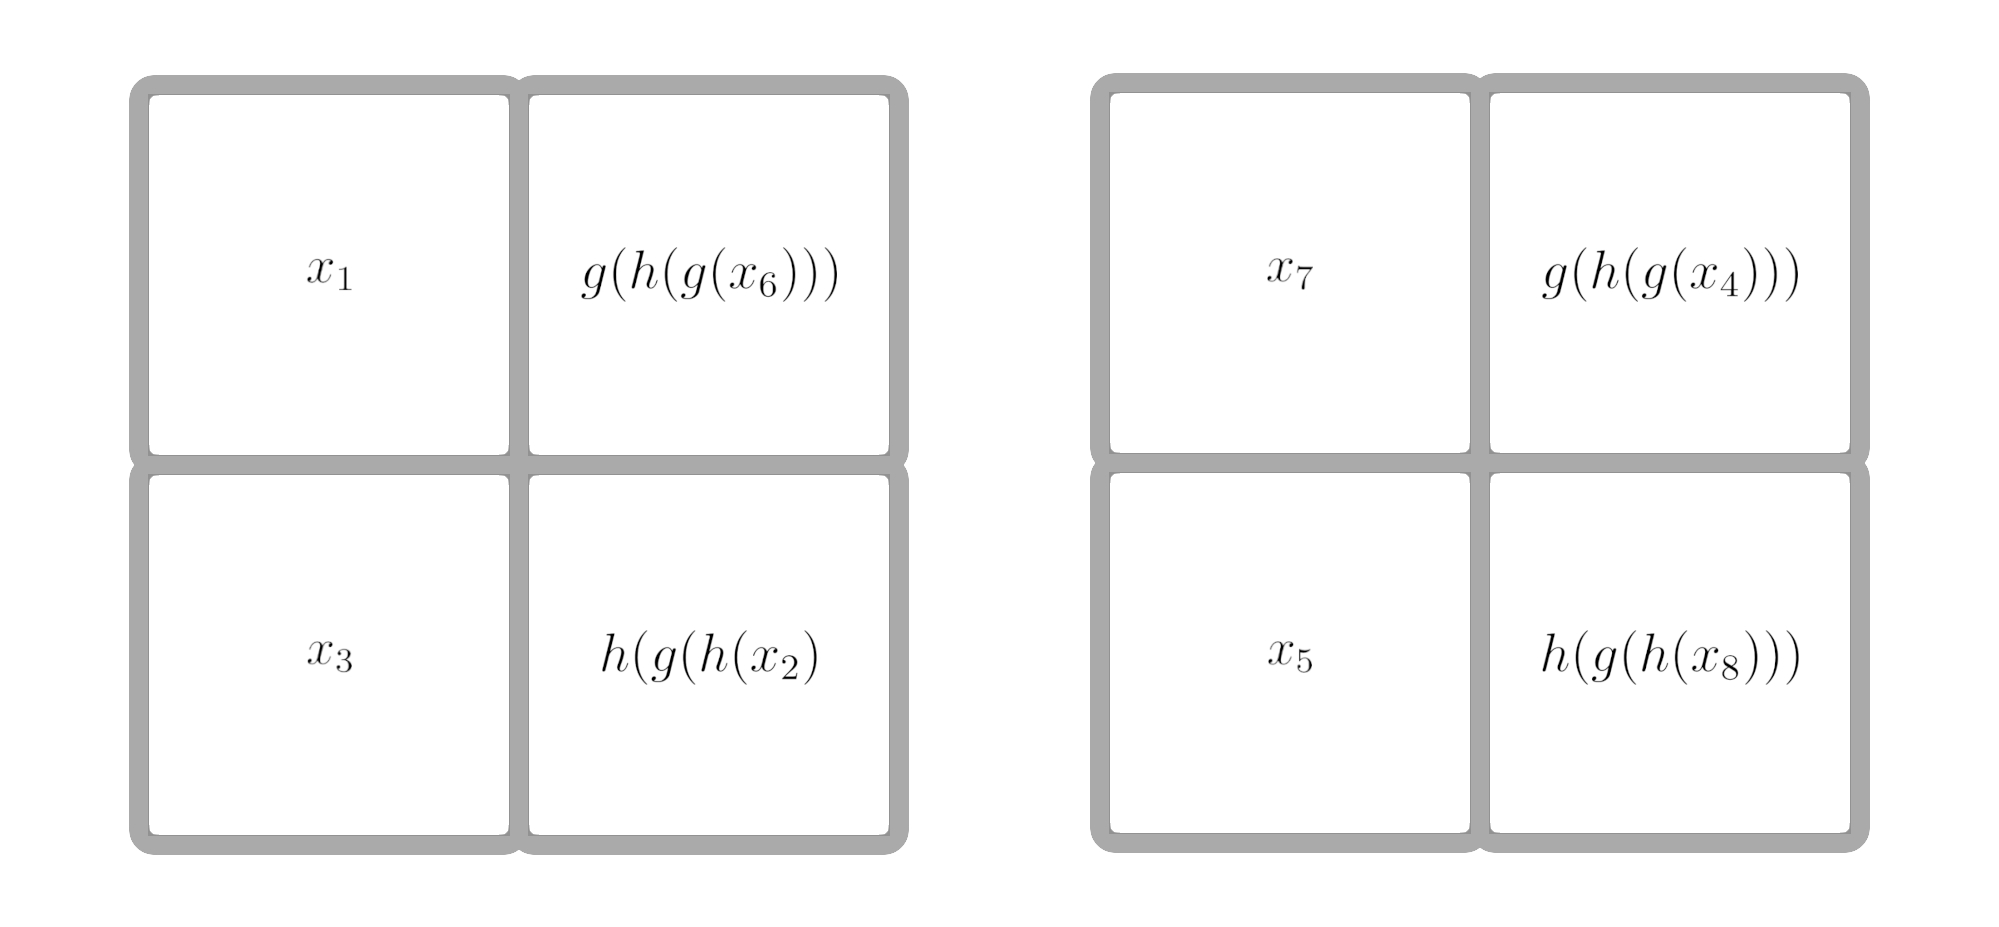
\includegraphics[scale=0.155]{Rhoch3.jpg}
\caption{Vector $x$ to $\gamma_R ( \gamma_R (\gamma_R(x)))$}
\end{figure}
\begin{figure}[H]
\centering
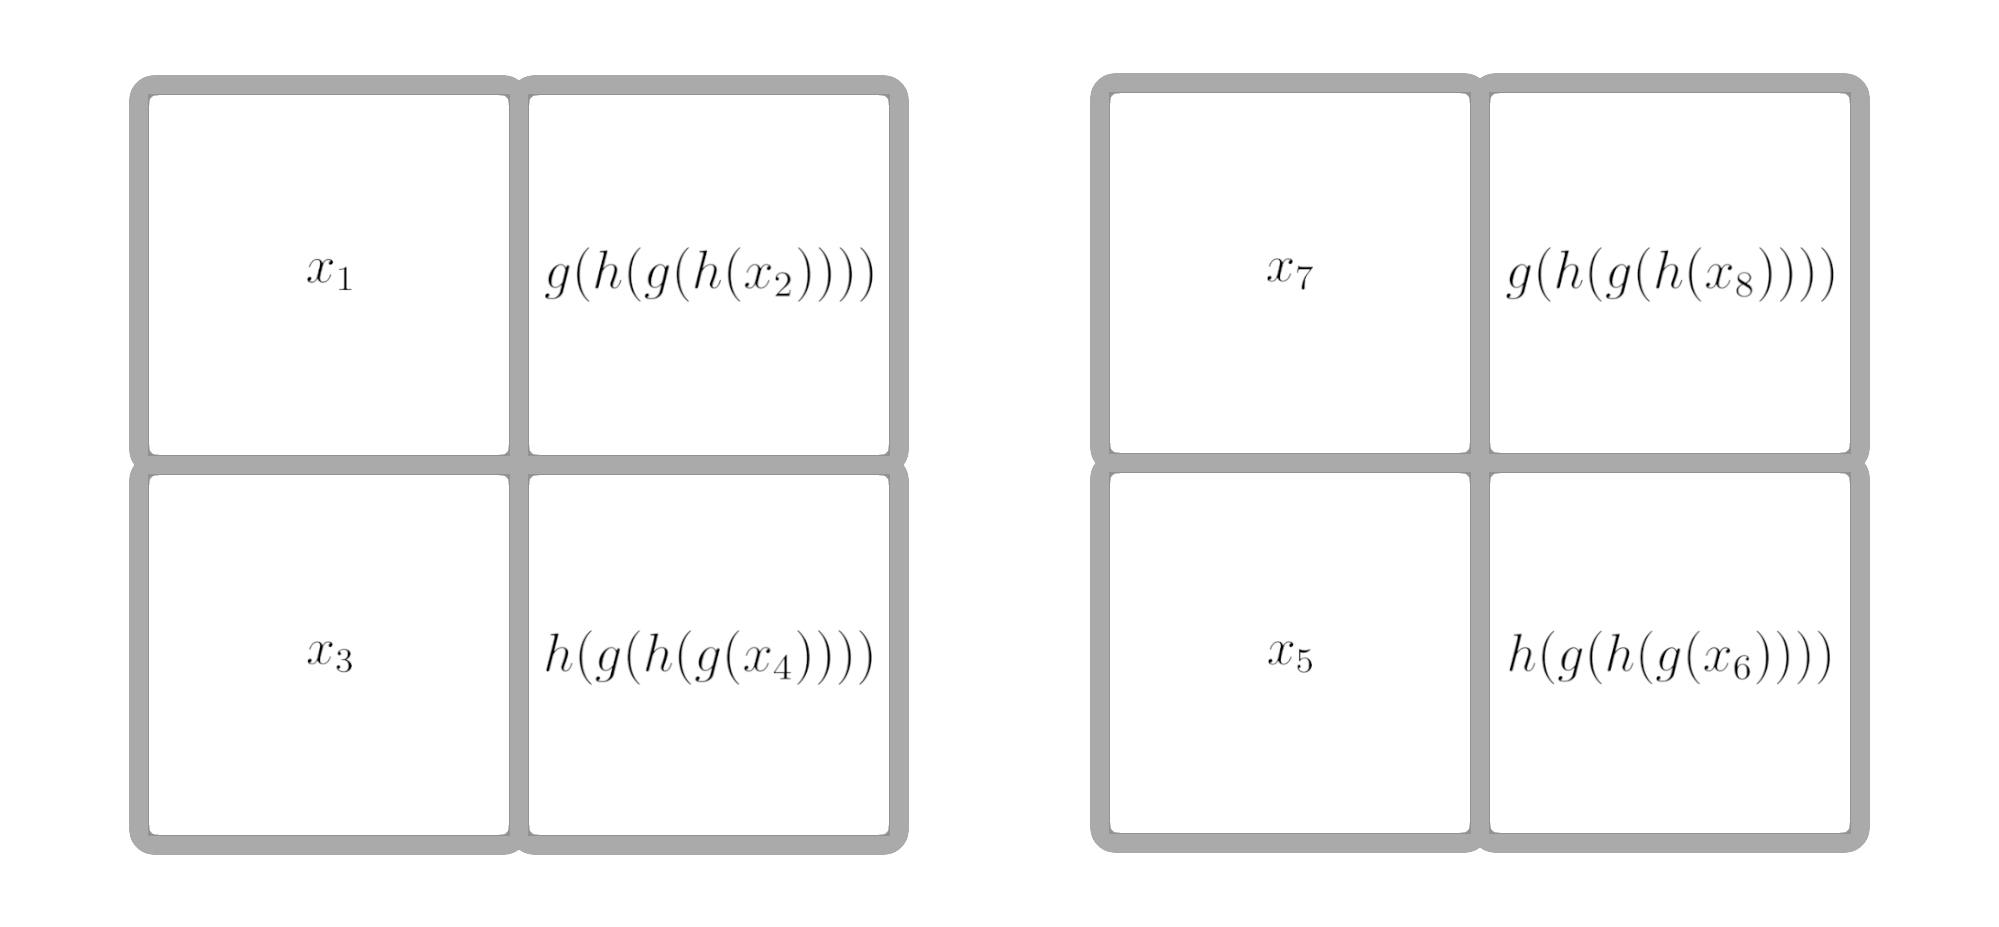
\includegraphics[scale=0.155]{Rhoch4.jpg}
\caption{Vector $x$ to $\gamma_R ( \gamma_R ( \gamma_R (\gamma_R(x))))$}
\end{figure}

Below, we can see the change in vector $x$ caused by the move $R^4$. The functions $g$ and $h$ are also nested when $\gamma_R$ is nested.
\begin{align*}
& \gamma_R (\gamma_R (\gamma_R (\gamma_R ((x_1, x_2, x_3, x_4, x_5, x_6, x_7, x_8  )))) \\
& =  (x_1, \ g(h(g(h(x_2)))), \ x_3, \ h(g(h(g(x_4)))), \ x_5, \ h(g(h(g(x_6)))), \ x_7, \ g(h(g(h(x_8)))) )
\end{align*}
The other basic moves change the vector as follows when executed four times:
\begin{align*}
& \gamma_U ( \gamma_U ( \gamma_U ( \gamma_U \left( (x_1, x_2, x_3, x_4, x_5, x_6, x_7, x_8  ) \right) ) ) ) \\ 
& =  \left((x_1, x_2, x_3, x_4, x_5, x_6, x_7, x_8  ) \right) \\
\\ 
& \gamma_D ( \gamma_D ( \gamma_D ( \gamma_D \left( (x_1, x_2, x_3, x_4, x_5, x_6, x_7, x_8  ) \right) ) ) ) \\ 
& =  \left((x_1, x_2, x_3, x_4, x_5, x_6, x_7, x_8  ) \right) \\
\\ 
& \gamma_R (\gamma_R (\gamma_R (\gamma_R ((x_1, x_2, x_3, x_4, x_5, x_6, x_7, x_8  )))) \\
& =  (x_1, \ g(h(g(h(x_2)))), \ x_3, \ h(g(h(g(x_4)))), \ x_5, \ h(g(h(g(x_6)))), \ x_7, \ g(h(g(h(x_8)))) ) \\
\\
& \gamma_L \left( (x_1, x_2, x_3, x_4, x_5, x_6, x_7, x_8  ) \right) \\ 
& =  \left( (h(g(h(g(x_1)))), x_2, g(h(g(h(x_3)))), x_4, g(h(g(h(x_5)))), x_6, h(g(h(g(x_7)))), x_8) \right) \\ 
\\
& \gamma_F \left( (x_1, x_2, x_3, x_4, x_5, x_6, x_7, x_8  ) \right) \\ 
& =  \left( x_1, x_2, h(g(h(g(x_3)))), g(h(g(h(x_4)))), x_5, x_6, g(h(g(h(x_7)))), h(g(h(g(x_8)))) \right) \\
\\
& \gamma_B \left( (x_1, x_2, x_3, x_4, x_5, x_6, x_7, x_8  ) \right) \\ 
& =  \left( g(h(g(h(x_1)))), h(g(h(g(x_2)))), x_3, x_4, h(g(h(g(x_5)))), g(h(g(h(x_6)))), x_7, x_8 \right)
\end{align*}
It can be seen that the changes when the same move is executed four times always consist of the function nestings $g(h(g(h(x))))$ and $h(g(h(g(x))))$. \textbf{Therefore the following must be shown}:
\begin{minipage}[H]{0.5\textwidth}
	\begin{align*}
		g(h(g(h(x)))) = x
	\end{align*}
\end{minipage}
\begin{minipage}[H]{0.5\textwidth}
      \begin{align*}
			h(g(h(g(x)))) = x
	  \end{align*}
\end{minipage}

with
\begin{align*}
g(x)=(x + 2) \hspace*{-0.5em} \mod 3 \ \ \ \ \ \ \ \ \ \ \ \ h(x) = (x+1) \hspace*{-0.5em} \mod 3 
\end{align*}
\begin{proofcustom}
To do this, $g(h(x))$ and $h(g(x))$ are first calculated.

      \begin{align*}
		 & g(h(x)) \\
		= \ & g((x+1) \hspace*{-0.5em} \mod 3) \\
		= \ & ((x+1) \hspace*{-0.5em} \mod 3) +2 \hspace*{-0.5em} \mod 3  \\
		= \ & (x \hspace*{-0.5em} \mod 3) +1 +2 \hspace*{-0.5em} \mod 3  \\
		= \ & (x \hspace*{-0.5em} \mod 3) +3 \hspace*{-0.5em} \mod 3  \\
		= \ & ((x \hspace*{-0.5em} \mod 3) \hspace*{-0.5em} \mod 3  \\
		= \ & x \hspace*{-0.5em} \mod 3 \\
		= \ & x \\
	\end{align*}


      \begin{align*}
		 & h(g(x)) \\
		= \ & h((x+2) \hspace*{-0.5em} \mod 3) \\
		= \ & ((x+2) \hspace*{-0.5em} \mod 3) +1 \hspace*{-0.5em} \mod 3  \\
		= \ & (x \hspace*{-0.5em} \mod 3) +2 +1 \hspace*{-0.5em} \mod 3  \\
		= \ & (x \hspace*{-0.5em} \mod 3) +3 \hspace*{-0.5em} \mod 3  \\
		= \ & ((x \hspace*{-0.5em} \mod 3) \hspace*{-0.5em} \mod 3  \\
		= \ & x \hspace*{-0.5em} \mod 3 \\
		= \ & x \\
	\end{align*}
\end{proofcustom}
The expression $(x \hspace*{-0.5em} \mod 3)$ can be transformed into $x$ in this case, since $x \in \{0,1,2\}$.

Since, $g(h(x))=x$ and $h(g(x))=x$, the following also holds:
\begin{align*}
		g(h(g(h(x)))) = g(h(x)) = x \\
			h(g(h(g(x)))) = h(g(x)) = x \\
	  \end{align*}

Thus, for any cube configuration $(\sigma, x)$:
\begin{align*}
\forall \ Z \in \{U, D, R, L, F, B\} \ . \ (\sigma, x) \cdot Z^4 = (\sigma, x)
\end{align*}
This means that the following also applies to any cube configuration $(\sigma, x)$:
\begin{align*}
\forall \ Z \in \{U, D, R, L, F, B\}, n \in \mathbb{N}, n \hspace*{-0.5em} \mod 4 = 0 \ . \ (\sigma, x) \cdot Z^n = (\sigma, x)
\end{align*}

Accordingly, the move $Z^4$ or $Z^n$ (with $n \hspace*{-0.5em} \mod 4$ and one-element moves $Z$) is a representative of the equivalence class of the empty move and is therefore also a way to form the identity element $N$ of the group $(\Gtwo, \mathlarger{\scriptstyle*})$.

This also applies analogously to the rotations of the cube. In section, \ref{Section_RotationOfCube} the cube rotations were defined by two face rotations each. These are opposite layers that do not affect the same cubies. 
\newpage The quadruple rotations of the cube are defined as face rotations below:
\begin{alignat*}{4}
& Z_lZ_lZ_lZ_l && \Leftrightarrow \ \ &&  DDDD  && \ U^{-1} U^{-1} U^{-1} U^{-1} \\
& Z_rZ_rZ_rZ_r && \Leftrightarrow &&   UUUU  && D^{-1}D^{-1}D^{-1}D^{-1}\\
& Y_lY_lY_lY_l && \Leftrightarrow && LLLL &&  R^{-1}R^{-1}R^{-1}R^{-1} \\
& Y_rY_rY_rY_r && \Leftrightarrow &&  RRRR &&  L^{-1} L^{-1} L^{-1} L^{-1} \\
& X_lX_lX_lX_L && \Leftrightarrow && BBBB &&  F^{-1}F^{-1}F^{-1}F^{-1} \\
& X_rX_rX_rX_r && \Leftrightarrow && FFFF  && B^{-1}B^{-1}B^{-1}B^{-1}   \\
\end{alignat*}

Since all quadruple rotations consist of two quadruple face rotations, the transformations described above can be transferred to the rotations. The vector $x$ therefore remains unchanged even if the same function $\beta$ is executed four times. Thus, for any cube configuration $(\sigma, x)$ also holds:
\begin{align*}
\forall \ W \in \{X_l, X_r, Y_l, Y_r, Z_l, Z_r\} \ . \ (\sigma, x) \cdot W^4 = (\sigma, x)
\end{align*}